
\section{Methodology}
\label{sec:methodology}

Discrete mathematics and computer science often deal with different types of data abstractions and structures such as sets, trees, and graphs, where concepts like nodes and links are used to describe the topology of a collection of objects and manipulate their data \citep[e.g.,][]{Skiena_2008_Book}. In graphs, the data---sometimes also referred to as the payload---resides at the vertices or nodes who are connected through links or edges, which may or may not have an associated direction. A visibility graph is a special type of undirected graphs in which the links are straight lines connecting intervisible nodes; that is, straight lines that do not go across any obstacle while connecting nodes that can see each other in a physical space \citep{LozanoPerez_1979_CACM}. Visibility graphs have been mostly used in robotics for navigation path planning \citep[e.g.,][]{Huang_2004_Proc, Oommen_1987_JRA} but have also seen applications in other fields including urban studies, interior architecture, medicine, and geosciences \citep[e.g.,][]{Raman_2010_UE, Ahmadlou_2010_JNT, Varoudis_2014_JSS, Phillips_2015_ESR}.

In a relatively recent study, \citet{Lacasa2008} applied the concepts of visibility graphs to the representation and analysis of time series. Multiple applications have been found to this idea in fields such as economics \citep{Yang_2009_PA, Wang2012} and climatology \citep{Elsner_2009_GRL}. In this study, we are particularly interested in the application of visibility graphs to the analysis of seismic sequences \citep{Telesca2012}. In such an application, the nodes in the visibility graphs are considered to be seismic events distributed over time. For any seismic time series, two characteristics are attributed to each event: (a) its occurrence time, and (b) the value associated to the event, here considered as the magnitude. The obstacles in the time-magnitude space are the vertical lines (or sticks) between the time axis and the magnitude of the event. Two events are in connection, or visible to each other, whenever the magnitude stick of no other event interrupts their linear connection.

In mathematical form, events $i$ and $j$ are visible to each other if they satisfy the inequality
%
\begin{equation}
	\frac{y_i - y_p }{t_p - t_i} > \frac{y_i - y_j}{ t_j - t_i} \, ,
	\label{eq:vg}
\end{equation}
%
\noindent
where $y$ is the value associated with the event and $t$ is the time of the event. The index $p$ indicates any event occurring between events $i$  and $j$. It follows from this that the visibility graph generated from a time series holds the following conditions. Connectivity: each event is visible to the two events to its immediate right and left sides, if there is any. Directivity: the graph is considered undirected by definition; that is, the algorithm explaining the connections between events is developed without defining a direction for the links between the events. And invariance: scaling or time-shifting the series does not change the resulting visibility graph, provided the transformation is done under affine conditions \citep{Lacasa2008}.

Figure \ref{fig:vg} shows an example of a visibility graph for a portion of one of the magnitude-time series to be considered later in this study. \myrevision{In this application, the visibility graph analysis is one-dimensional (i.e., there is no actual physical space but simply events in a catalog), and the magnitude sticks play the role of virtual obstacles distributed along the time line as defined by the occurrence of the events, which represent the nodes of the graph}. For each event $i$ we compute the connectivity degree, $k$, which is the sum of the connections to all other events $j$ visible by the $i$th event. Events are often categorized in small magnitude bins with $\Delta M = 0.1$, and we plot the connectivity degree as a function of the bin magnitude. Note that two earthquakes with the same magnitude can have different $k$ values, which ultimately depend on the occurrence time of the event and whether the time-neighboring events are of a larger or smaller magnitude.

\begin{figure*}[t]
	\centering
	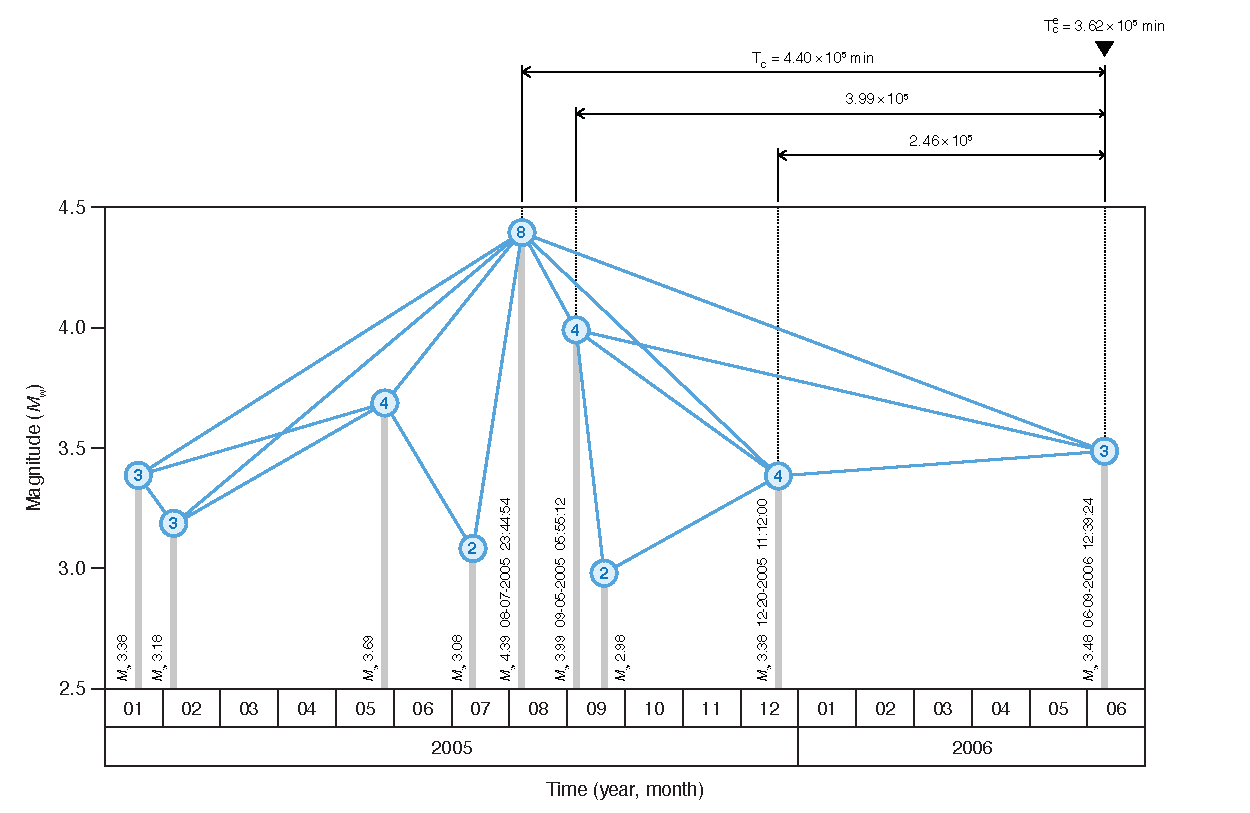
\includegraphics[width=0.8\textwidth]{figures/pdf/figure-01} 
	\caption{Illustration of the visibility graph method, as applied to a subset of events in a window of the magnitude-time series of the north Iranian seismic region of Kopeh Dagh. The events are identified by vertical thick lines (or sticks) on the horizontal time axis with size equal to the magnitude as indicated by the labels at the bottom of each stick. These sticks are considered to be the obstacles in the time-magnitude space where the graph resides. The visibility graph is composed by the nodes, represented with circles at the tip of each event stick, and the edges or links connecting them. The values inside each node correspond to the connectivity degree, $k$. This value indicates the number straight lines that can be draw between two (mutually visible) nodes without intersecting any obstacle (event stick). The values and time ranges shown at the top correspond to the time difference between events visible by the last event. These times are given in minutes and correspond to individual $T_c$ values. The mean $<$$T_c^e$$>$ value associated with this event is also shown at the top right. The mean value of all $<$$T_c^e$$>$ for the events in the graph is the window mean interval connectivity time, $<$$T_c^e$$>$. The color version of this figure is available only in the electronic edition.}
	\label{fig:vg}
\end{figure*}

% \myrevision{\color{red} In terms of earthquake catalog, the visibility graph studies the relation between earthquake events. Relation between small and large earthquakes are investigated in different studies. Lee et al (2009), based on developing LRCS model, in which is assumed that the occurrence of an earthquake leads to a release of energy with long range effects like in real earthquake fault systems, it has been known that earthquakes are long-range correlated. The visibility connections between the "hubs" (large events) and events even located very far on time could represent such long-range correlated behavior.}

\myrevision{It follows from this description that, for a given earthquake catalog, the visibility graph offers an alternative mathematical approach to study the correlations that exist between seismic events and their distribution (occurrence) in time. Such analysis can be explored in global terms (i.e., for all the events in a catalog), where long-range correlations might be more relevant in terms of the inter-visibility between large earthquakes, and the buildup of small earthquakes leading to greater magnitude events; or in local terms (i.e., for limited-time windows), where the occurrence of foreshocks and aftershocks may be more dominant. We explore such correlations in terms of how the properties of the visibility graph relate to the seismicity of the region.}

\myrevision{For instance,} plotting $k$ against magnitude results on a scattered set of points which have been shown to be acceptably represented by a linear regression. We refer to this correlation as the $k$-$M$ relationship. \myrevision{This is of relevance because it happens that, for a significant number of earthquake catalogs from distinctive seismic zones,} the slopes of the $k$-$M$ relationships show a linear regression with the seismicity $b$-value of the seismic zones under consideration. {This observation seems to hold} for a universal sample of $k$-$M$ slopes and $b$ values \myrevision{from different regions, as suggested by} \citet{Telesca2013, Telesca2014}. \citet{Telesca2014} also observed that it was reasonable to draw a relationship between the distribution of the events when considering whether these were connected (visible to each other) or not, and time. Let $T_c$ be the interval connectivity time, which is nothing but the time difference between two inter-visible events (see Fig.~\ref{fig:vg}); and $<$$T_c^e$$>$ the average of all $T_c$ values computed for event $e$; then it is possible to compute the visibility graph mean interval connectivity time $<$$T_c$$>$, which is the mean value of all $<$$T_c^e$$>$ in a given time sequence of events.

Because $<$$T_c$$>$ can be obtained for any sub-graph within a larger graph, that is, for any time window in a larger magnitude-time series of events, then it is possible to investigate the evolution of $<$$T_c$$>$ (and that of the $k$-$M$ slope and the $b$-value) for a moving window---with a constant number of events---sliding along the magnitude-time series. When doing so, \citet{Telesca2016} suggested to associate the values of each sub-sequence with the last event in the sub-sequence. Following this approach, \citet{Telesca2016} found that the variation of $<$$T_c$$>$ over time exhibited a possible relationship with the occurrence of earthquakes. This and the aforementioned relationship between the $k$-$M$ slope and the $b$-value are aspects we explore next for our region and years-interval of interest.

